\section{Methodology: Neutrino fluxes}
\subsection{Atmospheric neutrinos}
Atmospheric neutrinos are produced by the interaction of cosmic rays with the upper atmosphere. In the subsequent calculations we used the 3D Monte Carlo calculations by Honda \textit{et al.}~\cite{Honda:2011nf}. This model is based on the nuclear interaction model JAM used in Particle and Heavy-Ion Transport code System and modified DPMJET-III package. For neutrino fluxes with energy above 10\,GeV we use spectra by Sinegovskaya \textit{et al.}~\cite{Sinegovskaya:2014pia} which is computed by using Hillas-Gaisser cosmic ray spectra~\cite{Gaisser:2013ira} and Kimel-Mokhov hadronic model~\cite{Kalinovsky:1989kk} in semianalytical approach. Figures~\ref{ANspectra} and \ref{ANZAD} represent energy and zenith-angle distributions of atmospheric neutrino fluxes used in this paper.

\begin{figure}[htb!]
\begin{center}
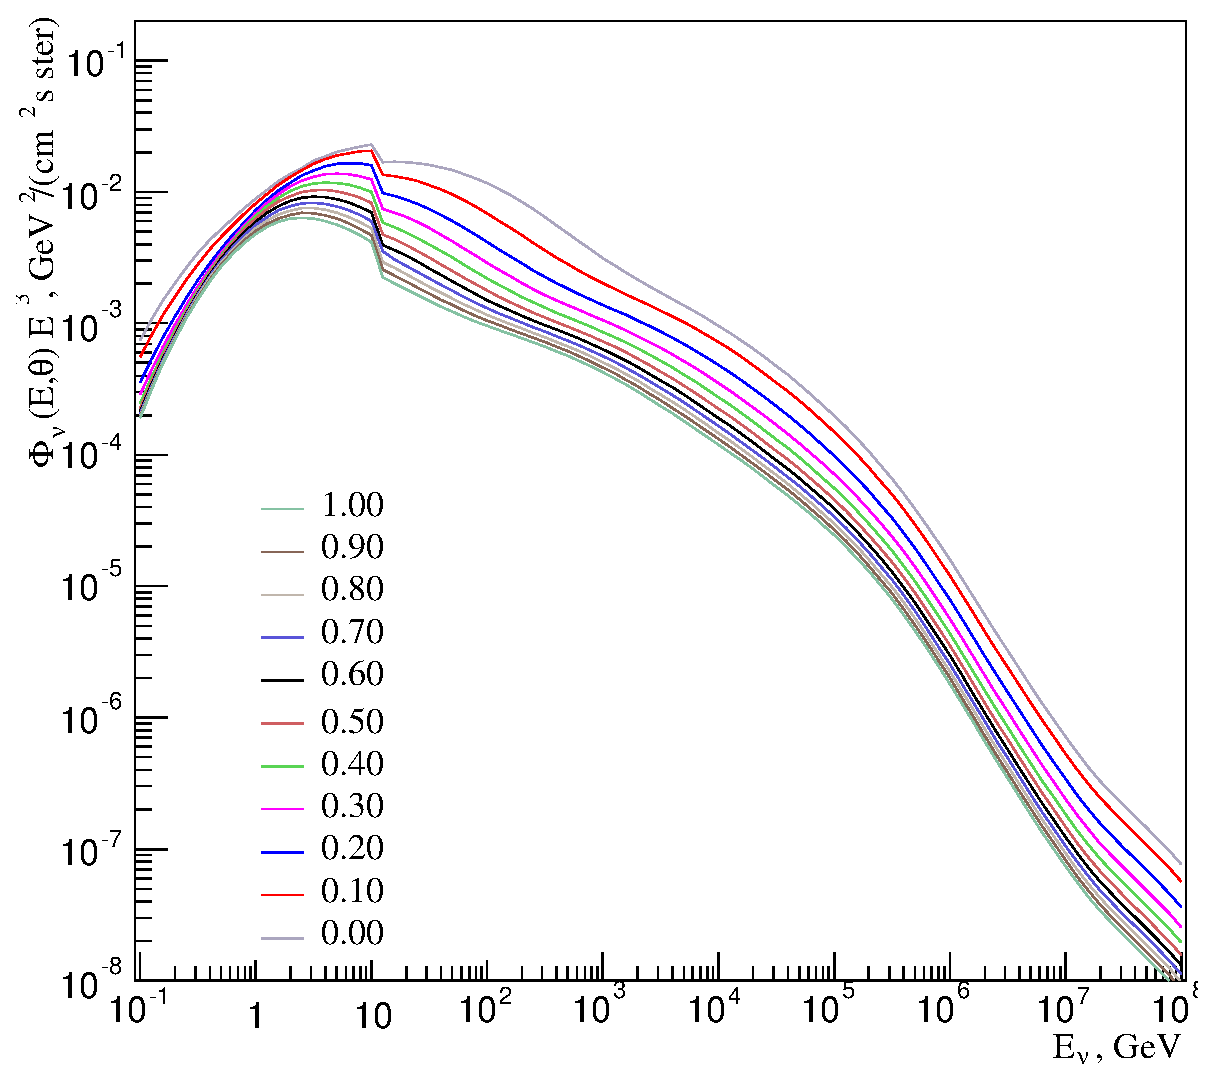
\includegraphics[width=0.45\textwidth]{./AN/HGm_KM_ne_spectra.eps}
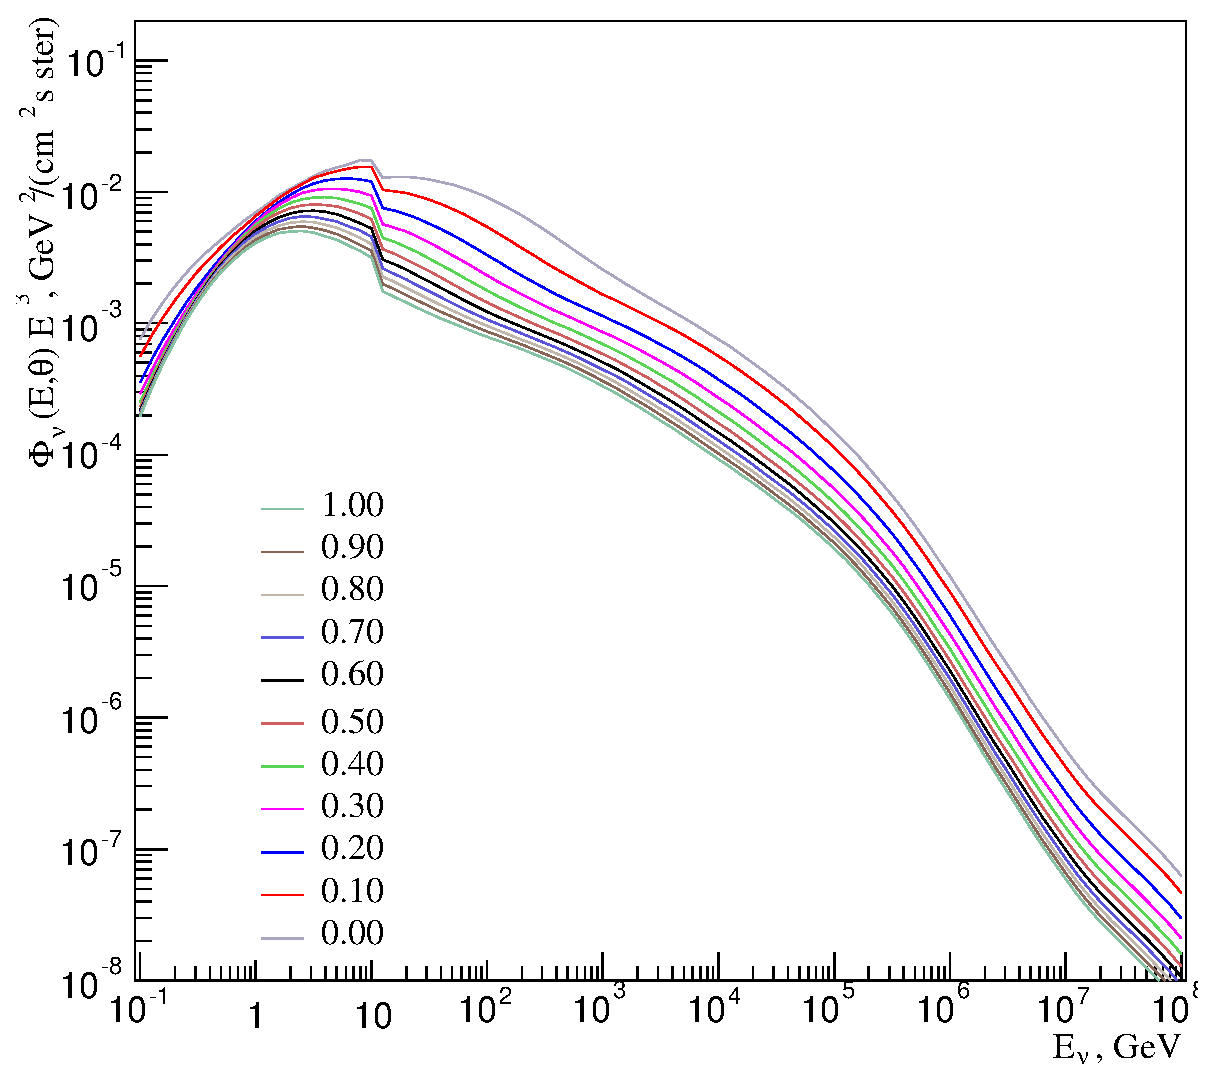
\includegraphics[width=0.45\textwidth]{./AN/HGm_KM_ae_spectra.eps}
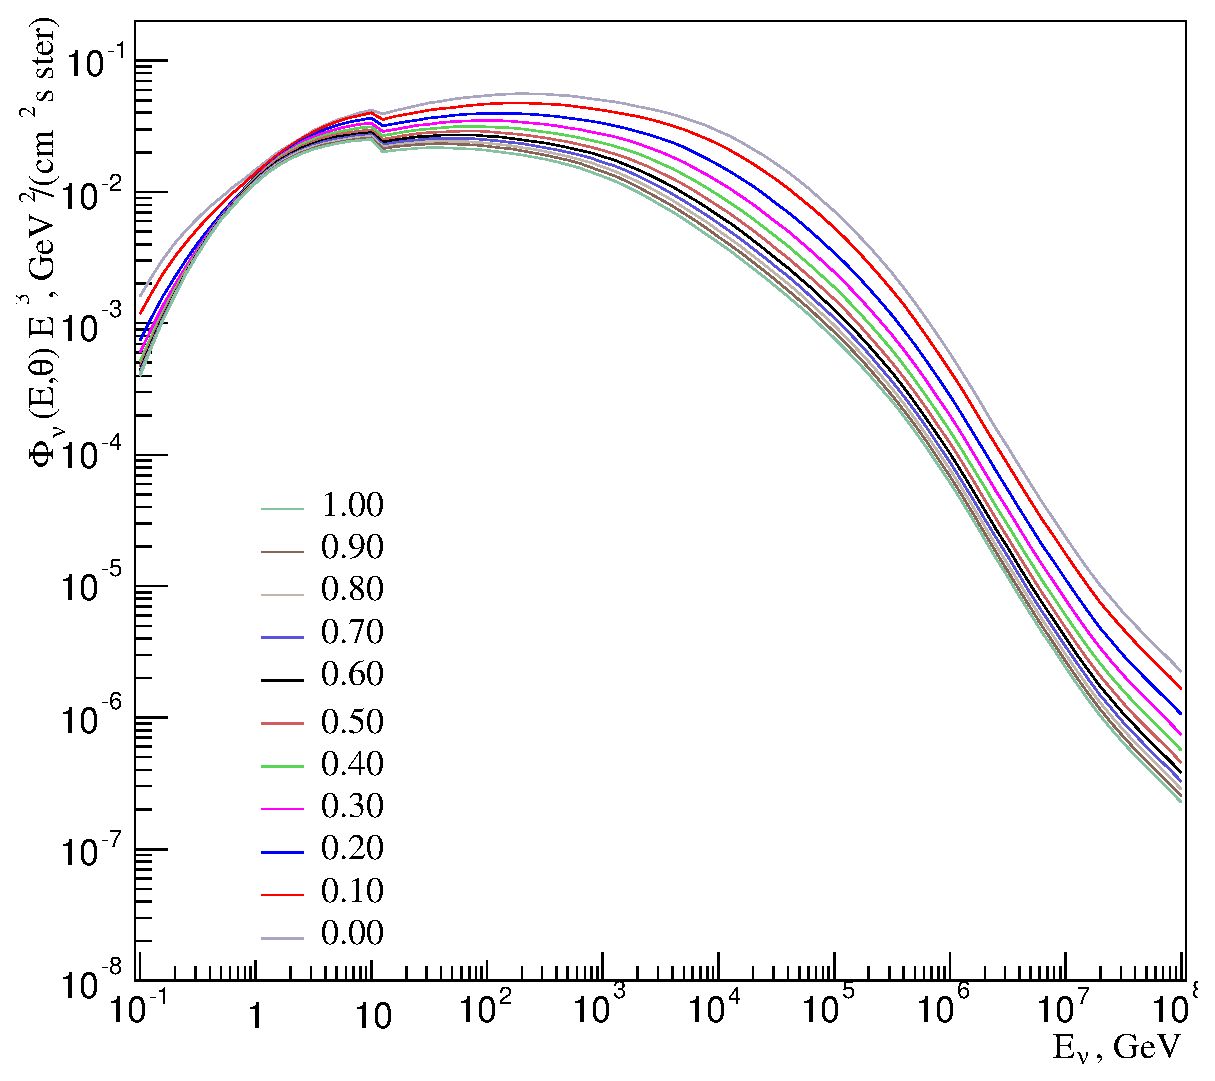
\includegraphics[width=0.45\textwidth]{./AN/HGm_KM_nm_spectra.eps}
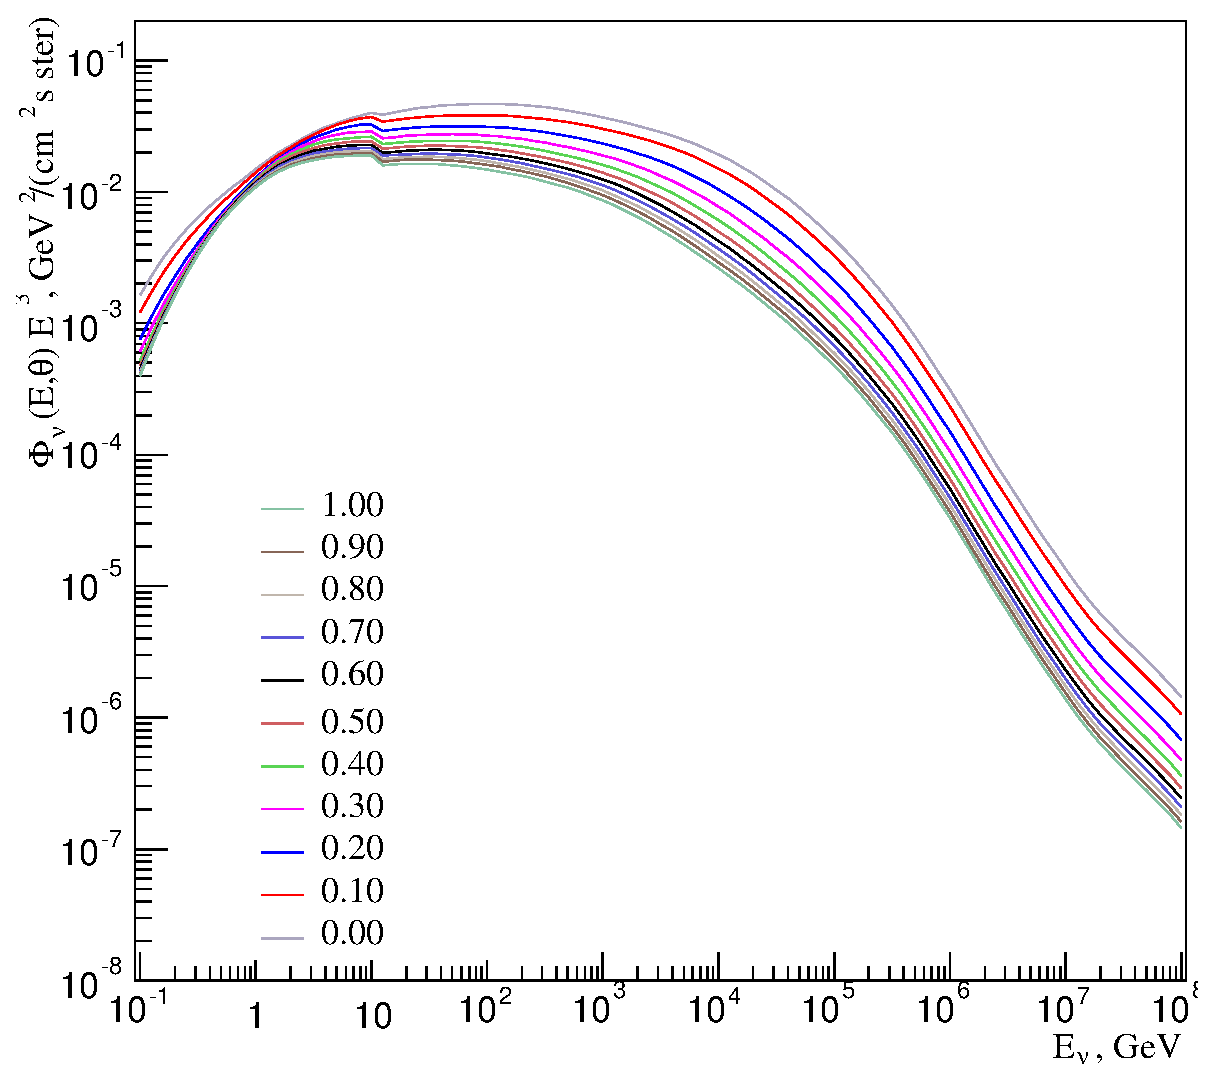
\includegraphics[width=0.45\textwidth]{./AN/HGm_KM_am_spectra.eps}
\caption{\label{ANspectra}Atmospheric neutrino energy spectra by Honda \textit{et al.}~\cite{Honda:2011nf} for $E_{\nu}$ from 100 MeV to 10 GeV and Sinegovskaya \textit{et al.}~\cite{Sinegovskaya:2014pia} for $E_{\nu}$ from 10 GeV to 100 PeV, used in this work}
\end{center}
\end{figure}

\begin{figure}[htb!]
\begin{center}
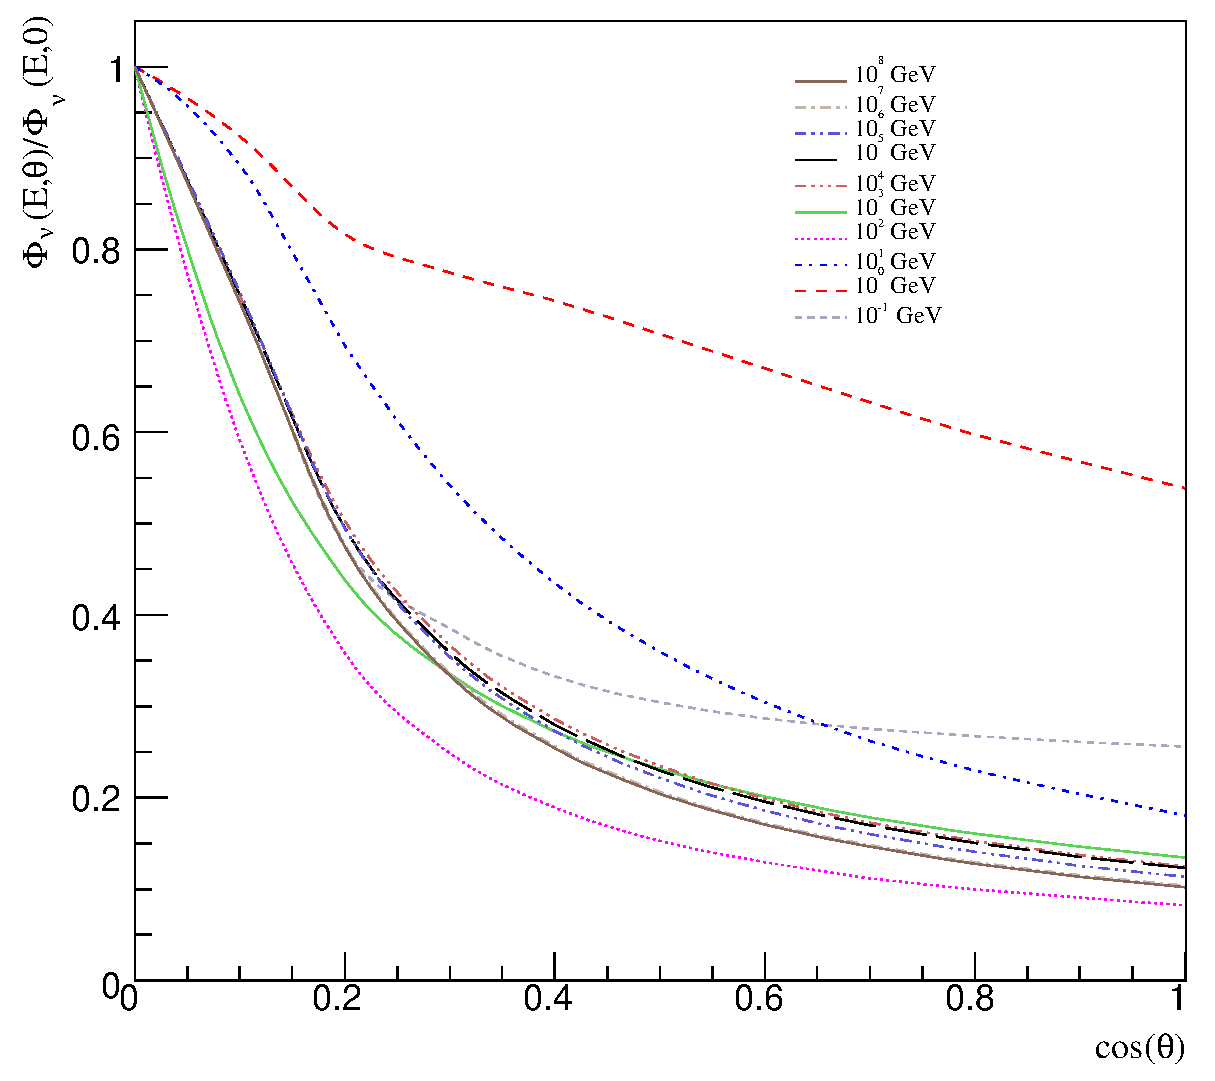
\includegraphics[width=0.45\textwidth]{./AN/HGm_KM_ne_ZAD.eps}
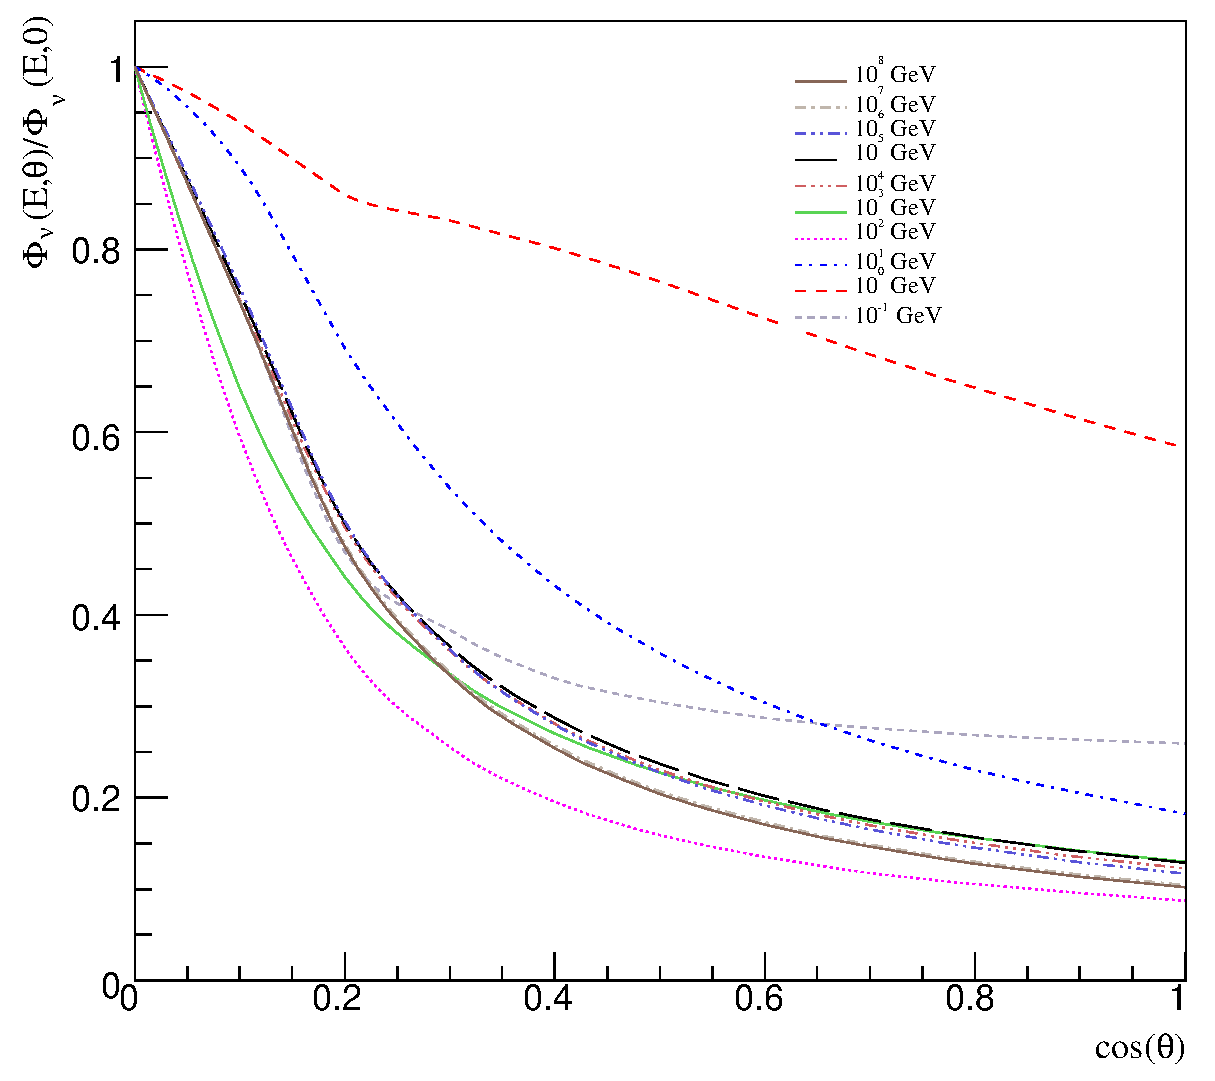
\includegraphics[width=0.45\textwidth]{./AN/HGm_KM_ae_ZAD.eps}
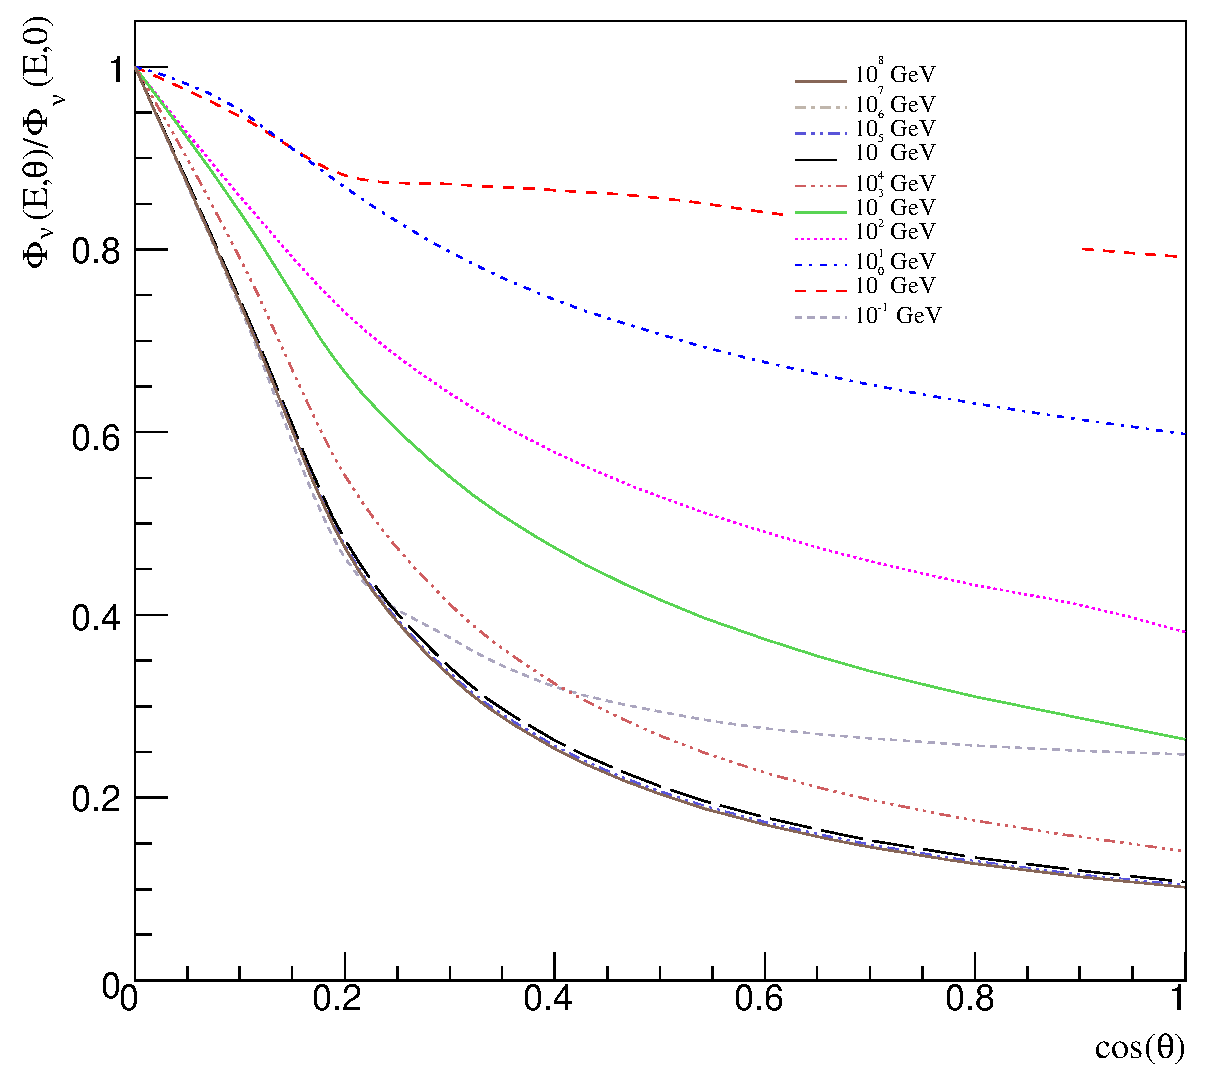
\includegraphics[width=0.45\textwidth]{./AN/HGm_KM_nm_ZAD.eps}
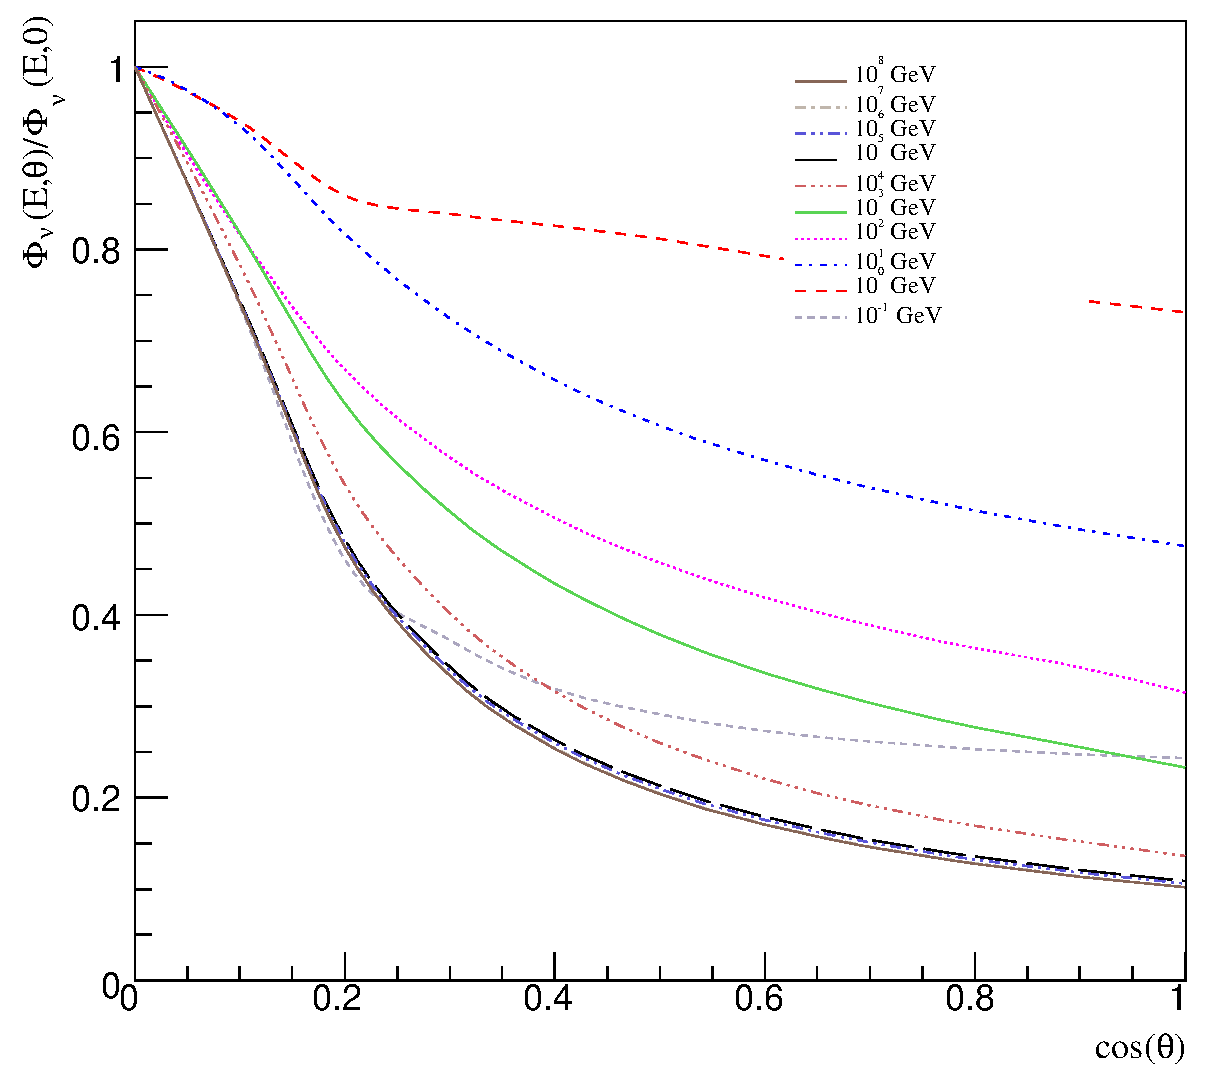
\includegraphics[width=0.45\textwidth]{./AN/HGm_KM_am_ZAD.eps}
\caption{\label{ANZAD}Zenith-angle distributions of atmospheric neutrino fluxes by Honda \textit{et al.}~\cite{Honda:2011nf} for $E_{\nu}$ from 100 MeV to 10 GeV and Sinegovskaya \textit{et al.}~\cite{Sinegovskaya:2014pia} for $E_{\nu}$ from 10 GeV to 100 PeV, used in this work}
\end{center}
\end{figure}

\subsection{Neutrino oscillations in medium}
Atmospheric neutrino fluxes are modified by neutrino oscillation phenomenon. For computing the flavor transition and survival probabilities we applied the result of the global neutrino oscillation data analysis (values of the neutrino mixing angles, CP violating phase and squared mass splittings) by Tortola \textit{et al.}~\cite{Tortola:2012te}.

Before getting the detector, atmospheric neutrinos pass through the body of the Earth. Therefore, we had to take into account the neutrino-matter coherent scattering (MSW effect). To solve the Wolfenstein equations describing the evolution of the neutrino system in a medium we decided to adopt the method from work~\cite{Naumov:2001ci}.

The density profile in the Earth in the presented calculations is described according to the Preliminary Reference Earth Model (PREM)~\cite{Dziewonski:1981xy} which contains 10 layers of density with various behaviour~\ref{PREM}. According to the method, each layer with varying density must be split into a number of sublayers of conditionally constant density. Hereby the process of neutrino propagating, from the moment of its birth in the sourse to the moment of entering the detector, may be considered as a process of consecutive propagations through a number of segments of relatively invariable density. Thus if ${S_{i}}$ is the evolution operator and the solution of Wolfenstein equation for the system of three mixed Dirac neutrinos passing through the $i$-th segment with constant density then $S=\prod{S_{i}}$ is the solution for the whole path from the source to the detector.

\begin{figure}[htb!]
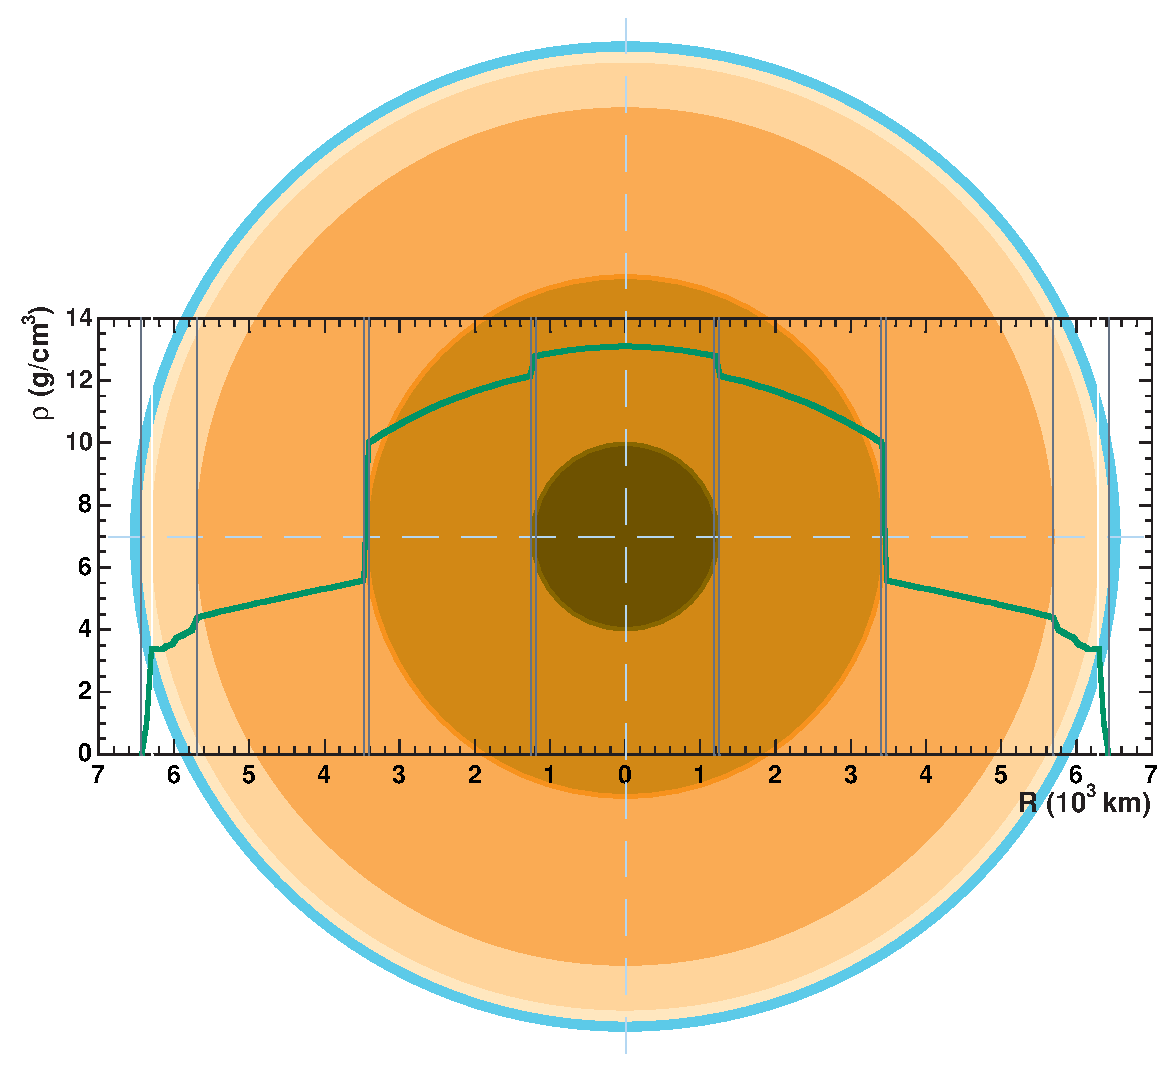
\includegraphics[width=0.5\textwidth]{./MSW/Earth_PREM.eps}
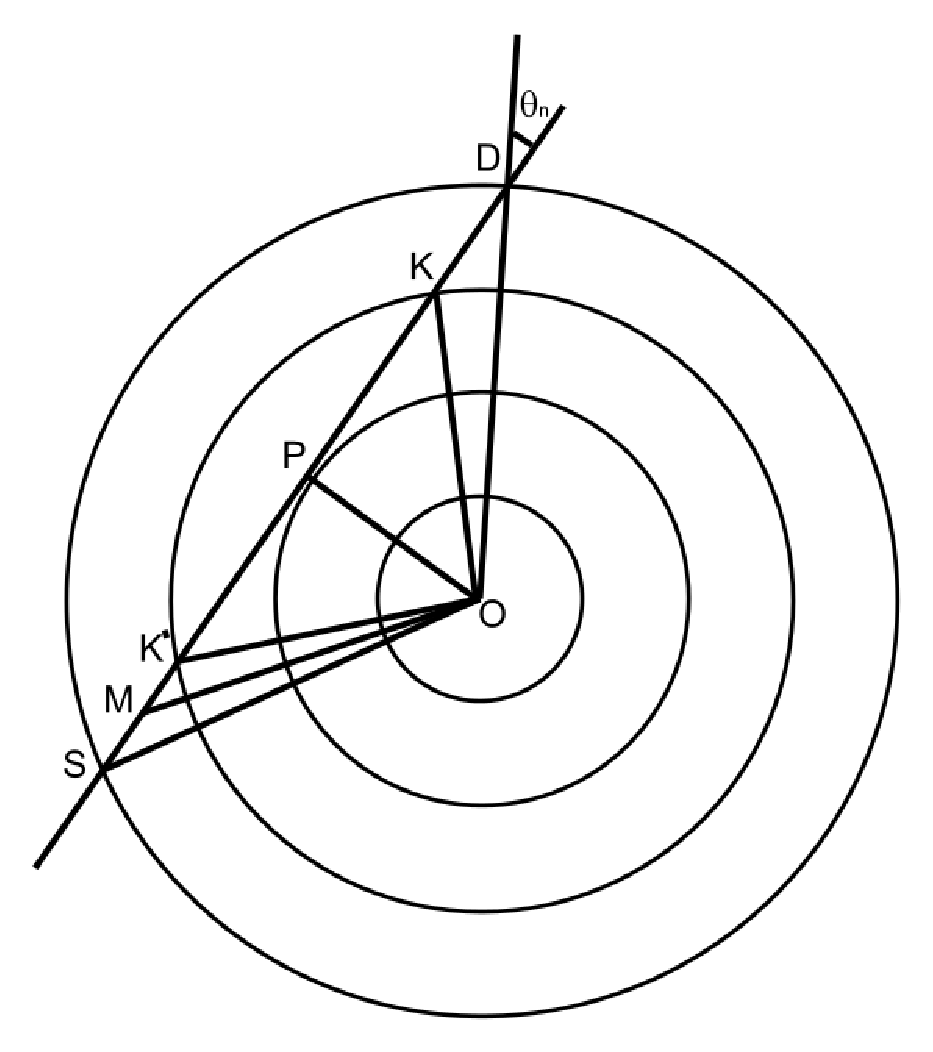
\includegraphics[width=0.5\textwidth]{./MSW/Earth_Layers.eps}
\caption{\label{PREM}Preliminary Reference Earth Model (PREM)~\cite{Dziewonski:1981xy} and the method of sublayers}
\end{figure}

The convenience of such method follows from the fact that independently of density distribution in a medium we have to find an exact solution of the equation for constant density only. Such solution has been obtained in work~\cite{Naumov:1991ju,Naumov:1991rh}. It is also worth noticing here that the number of sublayers in each layer is, by virtue of different thickness of such layers, individual and regulated by a convergence criterion for the method used. The criterion itself states that there're numbers ${N_{i}}$ of segments that each $i$-th layer is split into such that further increasing of these numbers doesn't change the values of probabilities within the desired accuracy. In our case these numbers can be established numerically only.

Examples of the neutrino oscillogramms in the Earth you can see in Fig.~\ref{ogramms}. Figure~\ref{modspectra} shows atmospheric neutrino spectra modulated neutrino oscillations in the Earth matter.

\begin{figure}[htb!]
\begin{center}
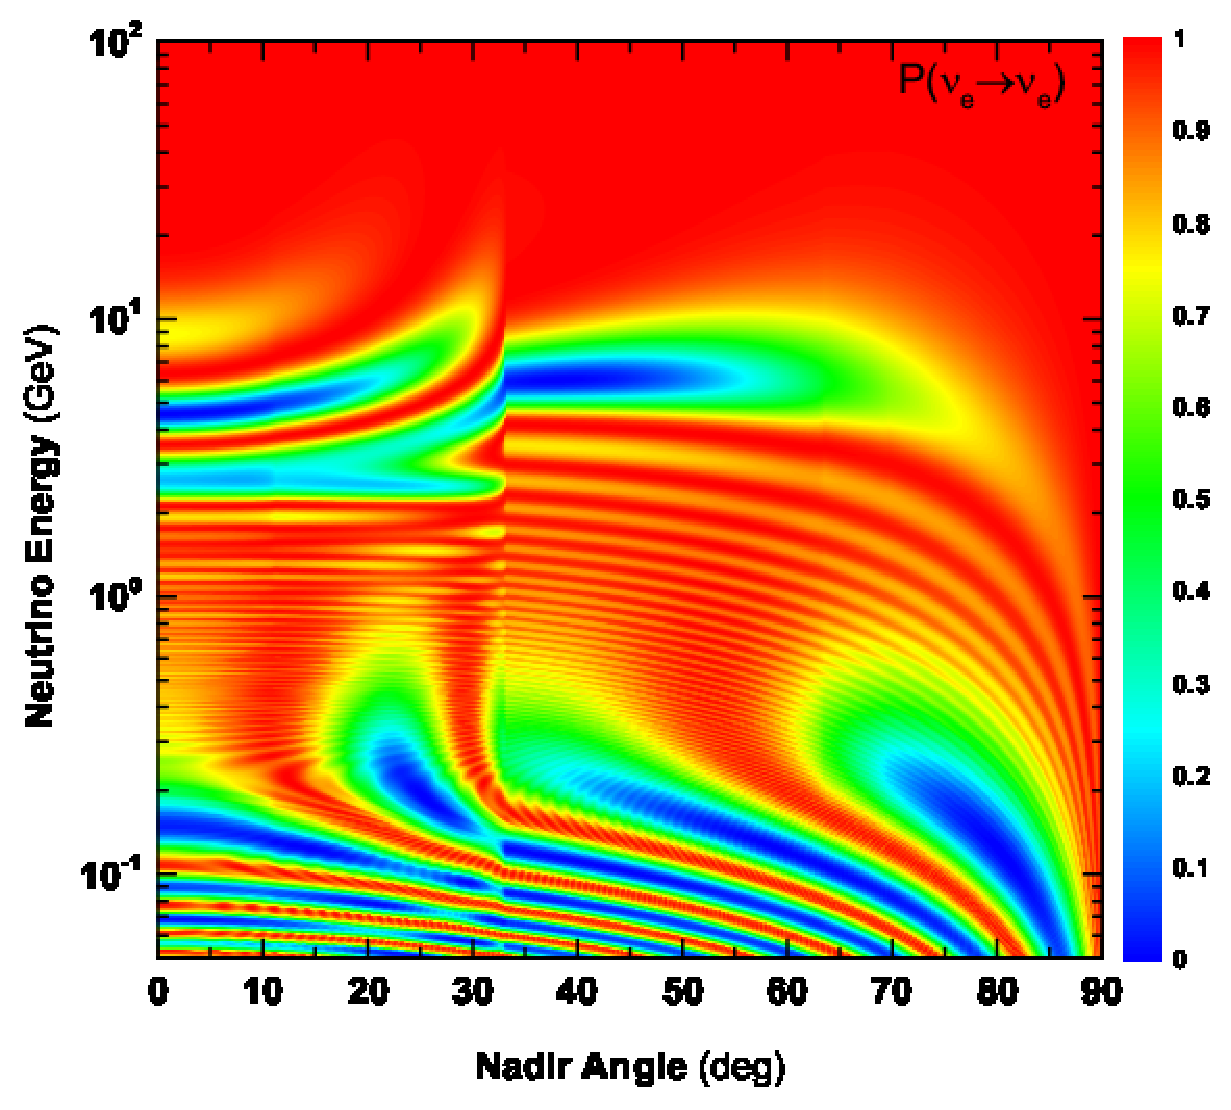
\includegraphics[width=0.3\textwidth]{./MSW/Pee-NH2.eps}
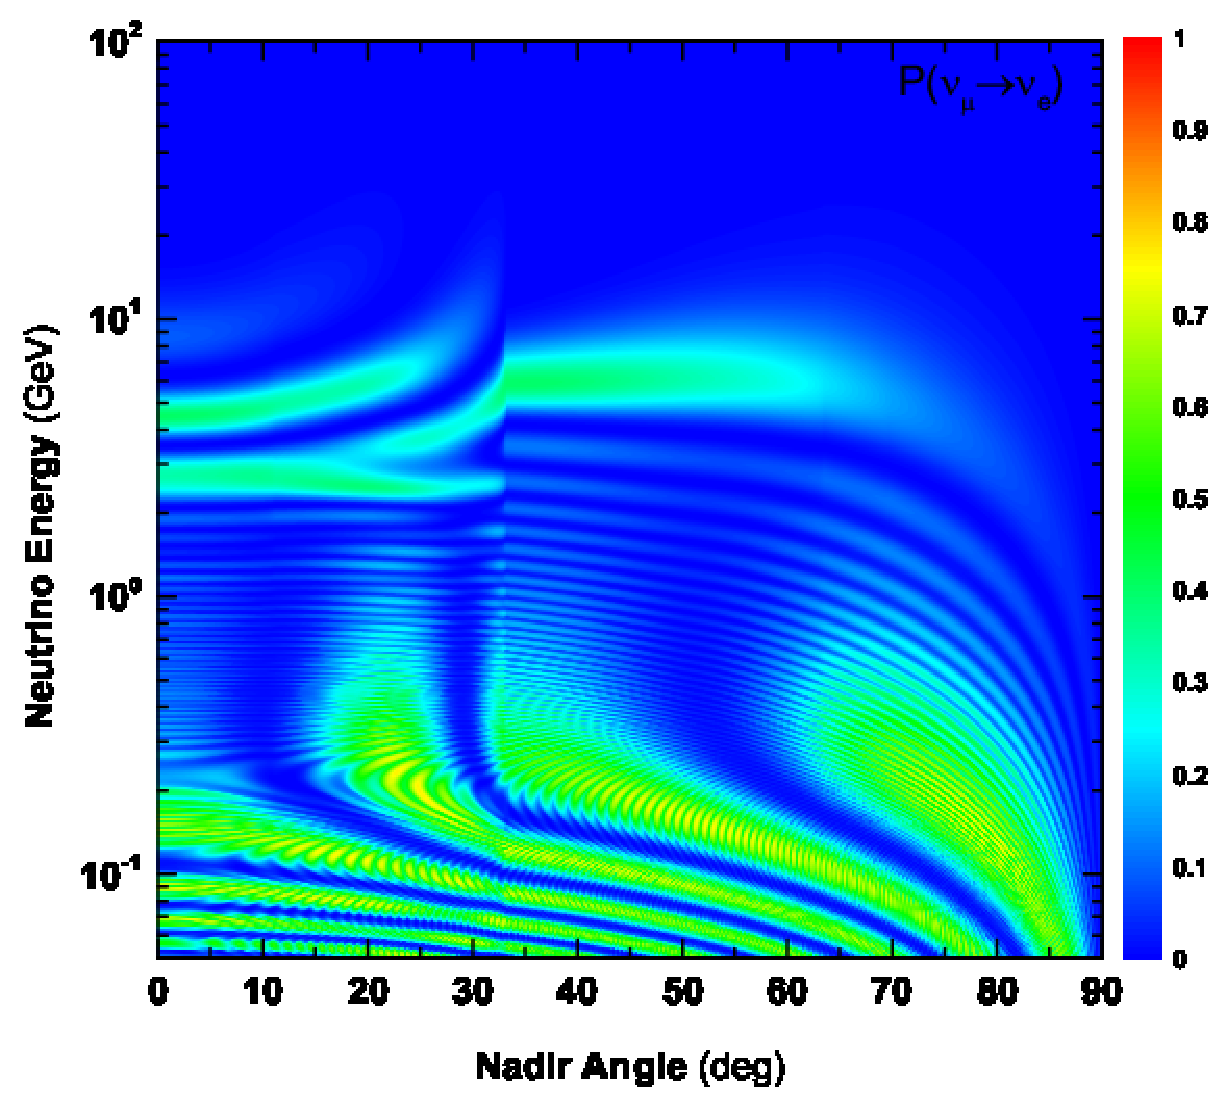
\includegraphics[width=0.3\textwidth]{./MSW/Pme-NH2.eps}
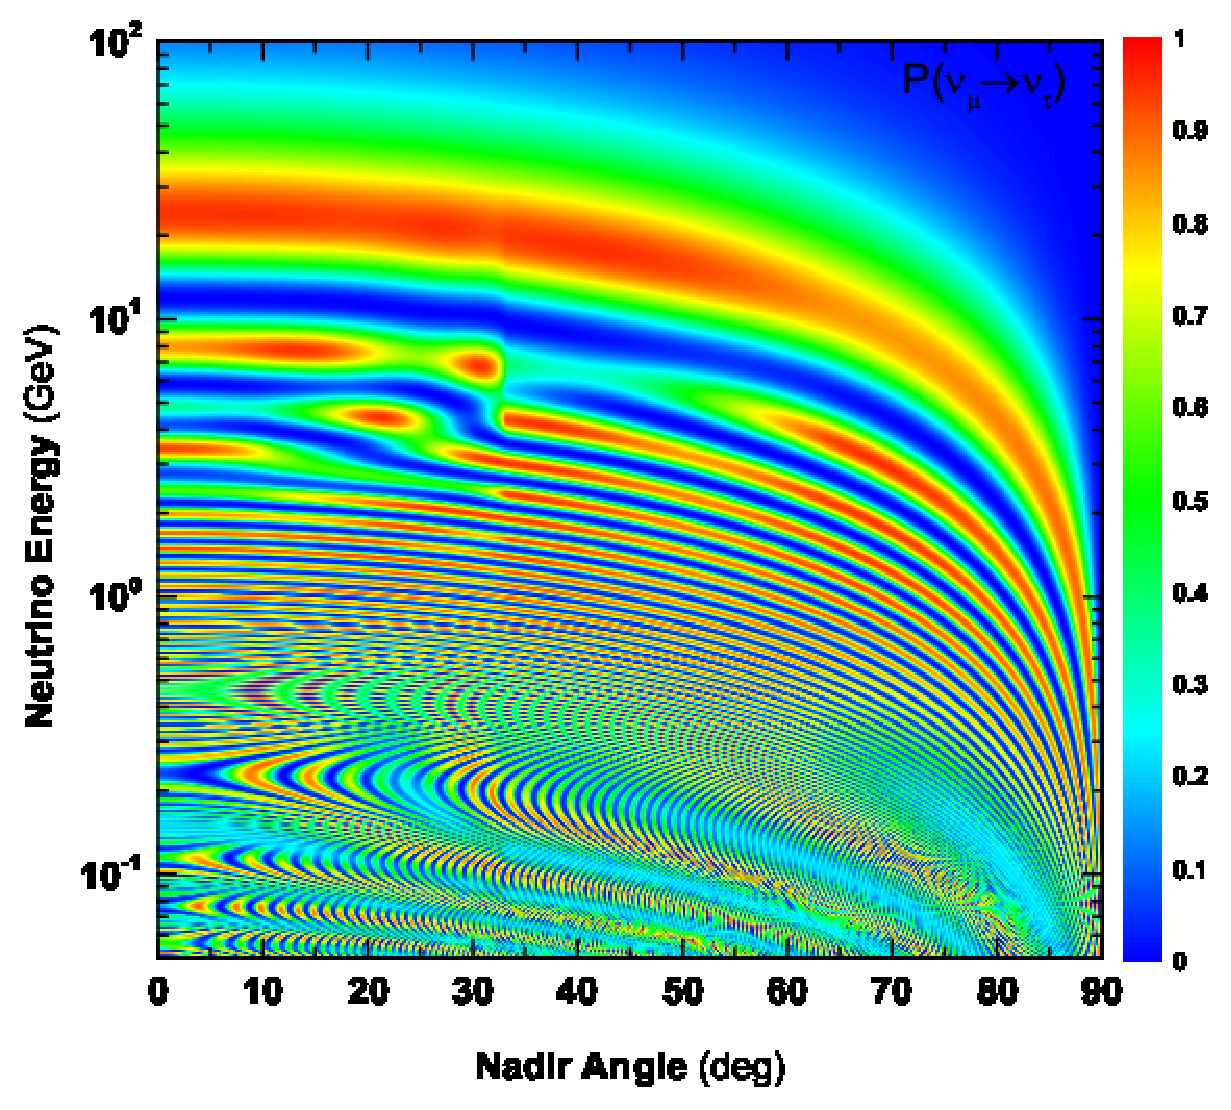
\includegraphics[width=0.3\textwidth]{./MSW/Pmt-NH2.eps}
\caption{\label{ogramms}\textbf{Neutrino oscillogramms} in the Earth for the case of normal neutrino mass, left to right: $\nu_{e}$ survival probability plot, $P_{\nu_{\mu}}\to{}P_{\nu_{e}}$, $P_{\nu_{\mu}}\to{}P_{\nu_{\tau}}$}
\end{center}
\end{figure}

\begin{figure}[htb!]
\begin{center}
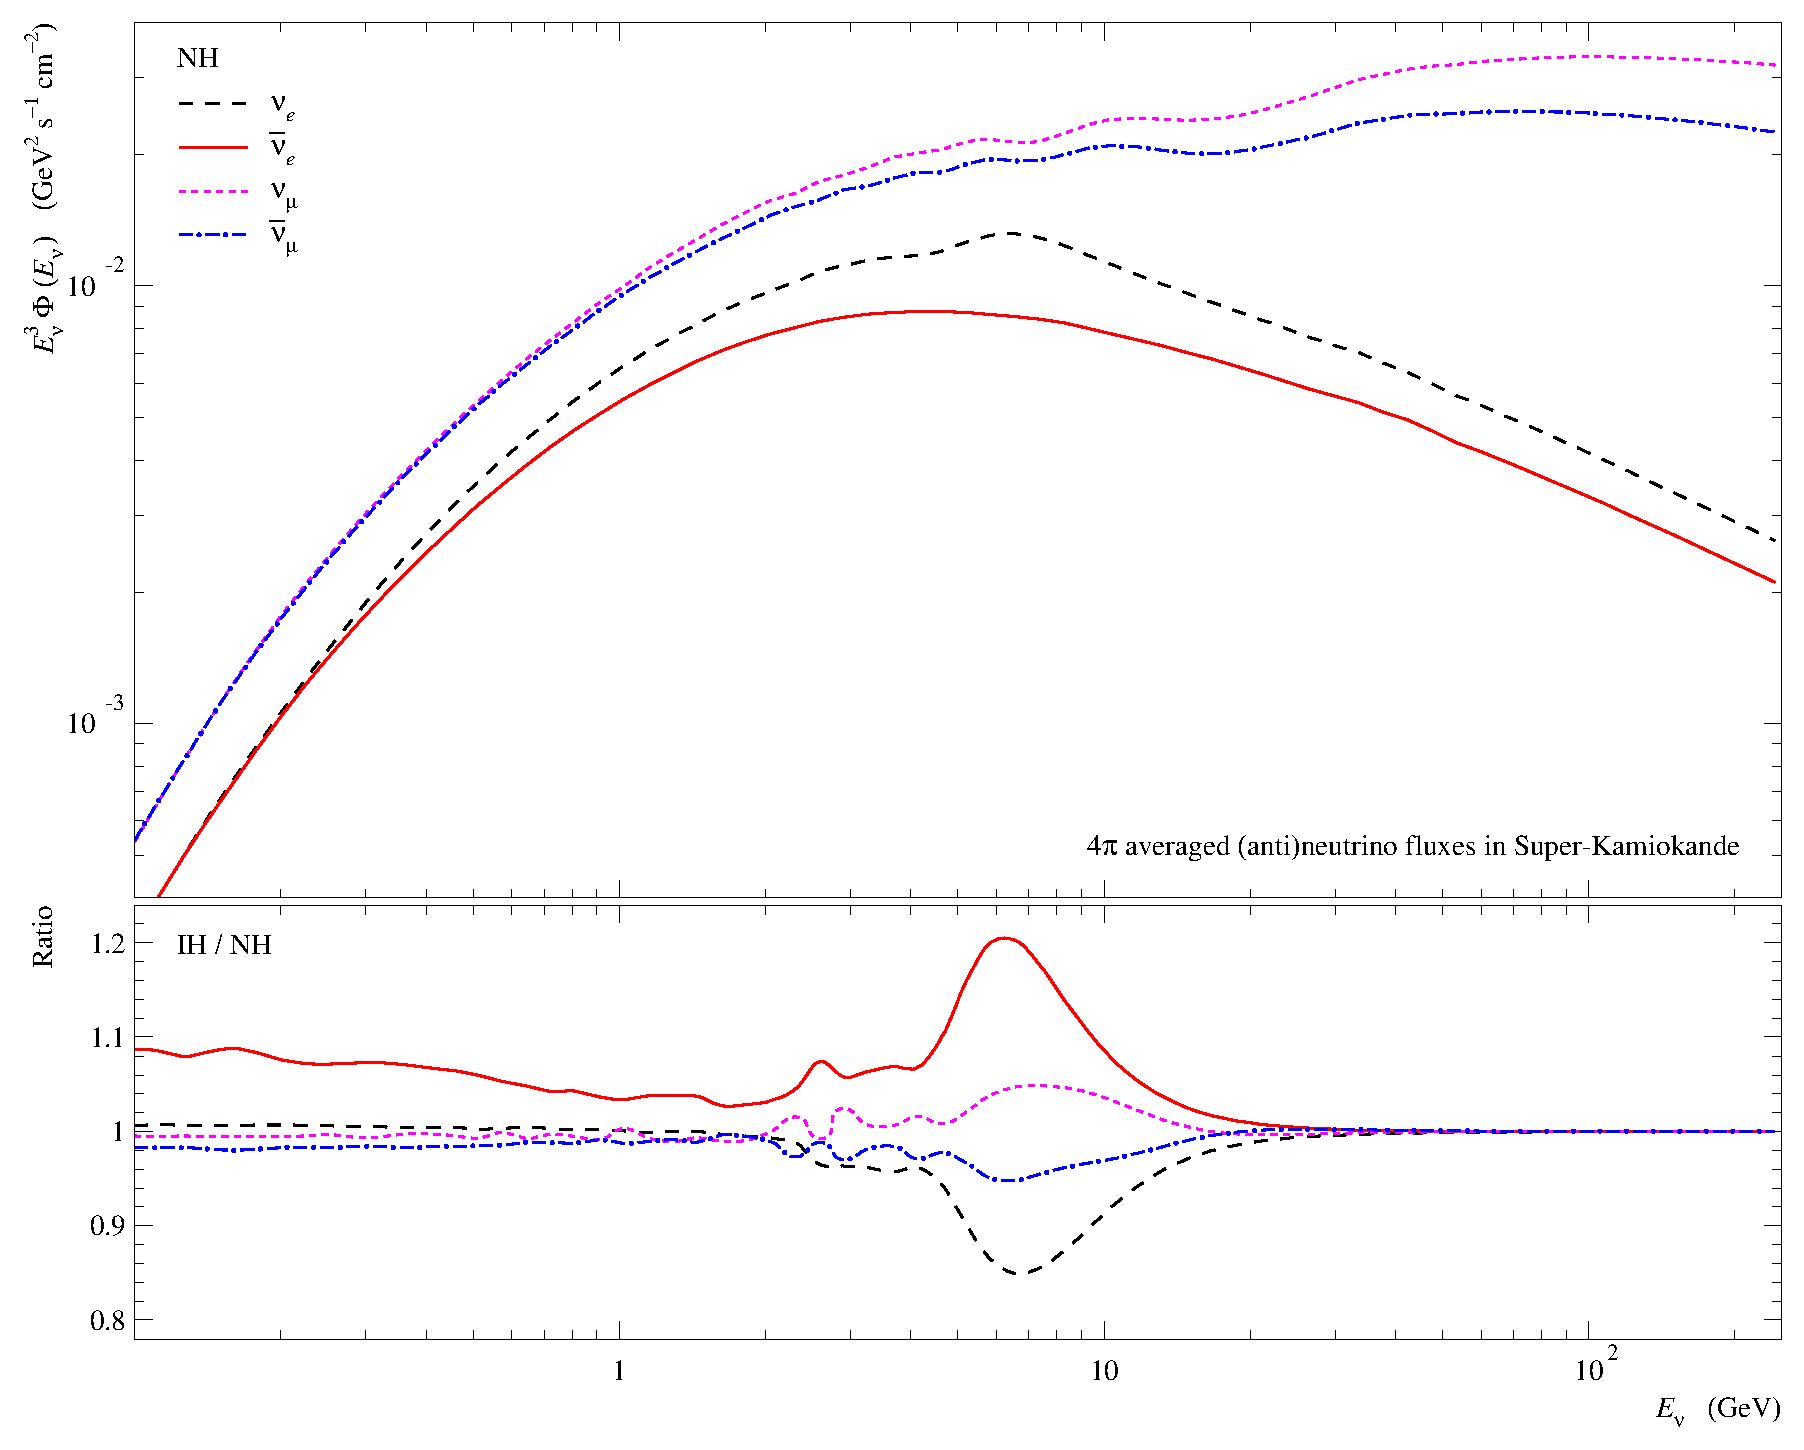
\includegraphics[width=0.6\textwidth]{./MSW/dF_dE_Honda11.eps}
\caption{\label{modspectra}\textbf{Flavor transition modulated} $4\pi$-averaged energy spectra of atmospheric neutrinos in Super-Kamiokande for the normal neutrino mass hierarchy (top panel) and the ratios of the energy spectra for the inverse mass hierarchy to these for the normal mass hierarchy (bottom panel)}
\end{center}
\end{figure}
